\BiChapter{环流的涨落定理}{Fluctuation theorems of cycle currents}

\BiSection{单环马氏链 LE 环流的涨落定理}{}
本章节将验证前面讨论的经验环流是否满足各类涨落定理。LE 经验环流的暂态涨落定理已经在文献 \cite{andrieux2007network} 中证明,不过该文中的证明还有些许不完整,下面先简述该文中关于单环马氏链的证明。记单环系统中两个 N 状态环为  $C^+ = (1,2,\cdots,N)$ 和 $C^- = (1,N,\cdots,2)$,令 $N^+_n$ 和 $N^-_n$ 分别表示 n 时刻环  $C^+$ 和 $C^-$ 分别形成的数量。由文献 \eqref{joint} 可以得到:
\begin{align*}
    &\;\mathbb{P}\left(N^+_n=k^+,N^-_n=k^-,N^c_n=k^c,\;\forall c\neq C^+,C^-\right)\\
    =&\; (\gamma^+)^{k^+}(\gamma^-)^{k^-}\prod_{c\neq C^+,C^-}
    \left(\gamma^c\right)^{k^c}\left|G_n(k^+,k^-,(k^c)_{c\neq C^+,C^-})\right|,
\end{align*}
其中 $\gamma^+ = p_{12}p_{23}\cdots p_{N1}$ 和 $\gamma^- = p_{1N}p_{N,N-1}\cdots p_{21}$ 分别是环 $C^+$ 和环 $C^-$中的转移概率的乘积,$G_n(k^+,k^-,(k^c)_{c\neq C^+,C^-})$ 表示所有容许轨迹的集合,这些轨迹满足 $C^+$ 形成 $k^+$ 次,$C^-$ 形成 $k^-$ 次,环 $c\neq C^+,C^-$ 形成 $k^c$ 次。上述方程可以重写为:
\begin{equation}\label{temp1}
    \mathbb{P}\left(N^+_n=k^+,N^-_n=k^-,\cdots\right)
    = (\gamma^+)^{k^+}(\gamma^-)^{k^-}\prod_{c\neq C^+,C^-}\left(\gamma^c\right)^{k^c}|G_n(k^+,k^-,\cdots)|.
\end{equation}
类似地, 如果交换上式中的 $k^+$ 和 $k^-$,可以得到
\begin{equation}\label{temp2}
\mathbb{P}\left(N^+_n=k^-,N^-_n=k^+,\cdots\right)
= (\gamma^+)^{k^-}(\gamma^-)^{k^+}\prod_{c\neq C^+,C^-}\left(\gamma^c\right)^{k^c}|G_n(k^-,k^+,\cdots)|.
\end{equation}
文献 \cite{andrieux2007network} 中的证明是基于 $G_n(k^+,k^-,\cdots)$ 与
$G_n(k^-,k^+,\cdots)$ 之间的一一对应关系的,即对 $G_n(k^+,k^-,\cdots)$ 的任意轨迹 $(\xi_0,\xi_1,\cdots,\xi_n)$ 都可以在 $G_n(k^-,k^+,\cdots)$ 中找到对应的逆轨迹  $(\xi_n,\xi_{n-1},\cdots,\xi_0)$。也就是说轨迹中环 $C^+$ 形成 $k^+$ 次,环$C^-$ 形成 $k^-$ 次,相应的逆轨迹中环 $C^+$ 形成 $k^-$ 次,环$C^-$ 形成 $k^+$ 次。同时也可得到两个集合中的元素数量相同,即:
\begin{equation}\label{equal}
    |G_n(k^+,k^-,\cdots)| = |G_n(k^-,k^+,\cdots)|.
\end{equation}
结合 \eqref{temp1},\eqref{temp2},和\eqref{equal},可以得到 LE 经验环流的暂态涨落定理:
\begin{equation}\label{theorem:transient fluatuation}
	\mathbb{P}\left(N^+_n=k^+,N^-_n=k^-,\cdots\right)
	= \mathbb{P}\left(N^+_n=k^-,N^-_n=k^+,\cdots\right)\left(\frac{\gamma^+}{\gamma^-}\right)^{k^+-k^-}.
\end{equation}
然而,上面也指出直观的想法是基于周期边界条件。例如,表\ref{example} 中的四状态单环系统的轨迹,其中环 $C^+$ 形成一次,然而相应的反环并没有形成$C^+$ 和 $C^-$。这说明逆轨迹并没有 $G_n(k^+,k^-,\cdots)$ 和 $G_n(k^-,k^+,\cdots)$ 之间的一一对应关系。
\begin{table}[htb!]
\renewcommand\arraystretch{1.3}\centering
\begin{tabular}{cccccccccc} \hline\hline
$n$                 & 0   & 1     & 2       & 3         & 4         & 5         & 6     & 7       \\ \hline
trajectory          & 1   & 2     & 3       & 4         & 4         & 1         & 4     & 3       \\ \hline
derived chain       & [1] & [1,2] & [1,2,3] & [1,2,3,4] & [1,2,3,4] & [1]       & [1,4] & [1,4,3] \\ \hline
cycles formed       &     &       &         &           & (4)       & (1,2,3,4) &       &         \\ \hline\hline
$n$                 & 0   & 1     & 2       & 3     & 4     & 5     & 6     & 7       \\ \hline
reversed trajectory & 3   & 4     & 1       & 4     & 4     & 3     & 2     & 1       \\ \hline
derived chain       & [3] & [3,4] & [3,4,1] & [3,4] & [3,4] & [3]   & [3,2] & [3,2,1] \\ \hline
cycles formed       &     &       &         & (1,4) & (4)   & (3,4) &       &         \\ \hline\hline
\end{tabular}
\caption{环擦除方式形成环的例子}\label{example}
\end{table}
通过上述论证,确实可以通过假设周期边界条件简化,简化论证。只是逆轨迹无法做到两个集合之间的一一映射,但这并不能否认暂态涨落定理 \eqref{theorem:transient fluatuation} 是错误的。在附录 E 中,给出了暂态涨落定理的严格证明。该证明的出发点是式 \eqref{trajectories} 中 $|G_n(k)|$ 的非平凡对称性。因为证明过于复杂,所以放在附录部分。这表明 LE 经验环流的联合分布满足一种非平凡对称性。

通过暂态涨落定理,可以进一步得到其他两种涨落定理。首先,回顾 LE 经验环流的矩母函数:
\begin{equation*}
    g_n(\lambda^+,\lambda^-,\cdots)
    = \mathbb{E}\left[e^{\lambda^+N^+_n+\lambda^-N^-_n+\sum_{c\neq C^+,C^-}\lambda^cN^c_n}\right].
\end{equation*}
可以得出 Kurchan-Lebowitz-Spohn 类型的涨落定理成立:
\begin{align*}
    g_n(\lambda^+,\lambda^-,\cdots)
    &= \sum_{k}e^{\sum_{c\in\mathcal{C}}\lambda^ck^c}\mathbb{P}\left(\cdots,N^+=k^+,N^-=k^-\right)\\
    &= \sum_{k}e^{\sum_{c\in\mathcal{C}}\lambda^ck^c}
    \mathbb{P}\left(\cdots,N^+=k^-,N^-=k^+\right)\left(\frac{\gamma^+}{\gamma^-}\right)^{k^+-k^-}\\
    &= \sum_{k}e^{\cdots+\left(\lambda^+-\log\frac{\gamma^+}{\gamma^-}\right)k^++
    \left(\lambda^--\log\frac{\gamma^-}{\gamma^+}\right)k^-}\mathbb{P}(\cdots,N^+=k^-,N^-=k^+)\\
    &= \mathbb{E}\left[e^{\cdots+\left(\lambda^--\log\frac{\gamma^+}{\gamma^-}\right)N^+_n+
    \left(\lambda^++\log\frac{\gamma^+}{\gamma^-}\right)N^-_n}\right]\\
    &= g_n\left(\lambda^--\log\frac{\gamma^+}{\gamma^-},
    \lambda^++\log\frac{\gamma^+}{\gamma^-},\cdots\right),
\end{align*}
其中 $\log(\gamma^+/\gamma^-)$ 是环 $C^+$ 的匹配度。接下来,考虑 n 趋于无穷是时,单环系统的极限情况,易知:
\begin{align*}
e^{-nI_J(\cdots,\nu^+,\nu^-)}
&\propto \mathbb{P}\left(\cdots,J^+_n\approx\nu^+,J^-_n\approx\nu^-\right)\\
&= \mathbb{P}\left(\cdots,J^+_n\approx\nu^-,J^-_n\approx\nu^+\right)
\left(\frac{\gamma^+}{\gamma^-}\right)^{n(\nu^+-\nu^-)}\\
&\propto e^{-n\left[I_J(\cdots,\nu^-,\nu^+)-\left(\log\frac{\gamma^+}{\gamma^-}\right)
(\nu^+-\nu^-)\right]}.
\end{align*}
这蕴含着下面 Gallavotti-Cohen 形式的涨落定理成立:
\begin{equation}\label{G-C type fluctuation}
    I_J(\cdots,\nu^+,\nu^-)=I_J(\cdots,\nu^-,\nu^+)-\left(\log\frac{\gamma^+}{\gamma^-}\right)(\nu^+-\nu^-).
\end{equation}

类似地,可以得到 LE 经验净环流的涨落定理。类似于章节 ~\ref{LELDP} 中讨论 $(\tilde{J}^c_n)_{c\in\mathcal{C}}$,只需关注环 $C^+$ 的经验净环流。令
$\tilde{g}_n(\lambda) = \mathbb{E}[e^{\lambda n\tilde{J}^+_n}]$ 为 $\tilde{J}^+_n$的矩母函数,$I_{\tilde{J}}(x)$为相应的速率函数。下面各种有关的涨落皆可得出:
1) 暂态涨落定理:
\begin{equation*}
\frac{\mathbb{P}(\tilde{J}^+_n=x)}{\mathbb{P}(\tilde{J}^+_n=-x)}
= \left(\frac{\gamma^+}{\gamma^-}\right)^{nx}.
\end{equation*}

2) Kurchan-Lebowitz-Spohn 类型的涨落定理:
\begin{equation*}
\tilde{g}_n(\lambda)=\tilde{g}_n\left(-\left(\lambda+\log\frac{\gamma^+}{\gamma^-}\right)\right).
\end{equation*}

3)积分涨落定理 : 取 $\lambda = -\log \gamma^+/\gamma^-$ 带入上式 2)可得
\begin{equation*}
\mathbb{E}\left[e^{\lambda n\tilde{J}^+_n}\right]=1.
\end{equation*}

4) Gallavotti-Cohen 类型的涨落定理:
\begin{equation*}
\tilde{I}_J(x)=\tilde{I}_J(-x)-\left(\log\frac{\gamma^+}{\gamma^-}\right)x.
\end{equation*}

最后考虑熵产生涨落和环流涨落之间的关系。回顾熵产生的定义 \cite{jiang2004mathematical}:
\begin{equation*}
	W_n=\frac{1}{2}\sum_{c\in\mathcal{C}}\tilde{J}^c_n\log\frac{\gamma^c}{\gamma^{c-}}=\tilde{J}^+_n\log\frac{\gamma^+}{\gamma^-}.
\end{equation*}
熵产生的暂态涨落定理可以整理为:
\begin{equation*}
	\frac{\mathbb{P}(W_n=x)}{\mathbb{P}(W_n=-x)}
	= \frac{\mathbb{P}(\tilde{J}^+_n=x/(\log\frac{\gamma^+}{\gamma^-}))}{\mathbb{P}(\tilde{J}^-_n=-x/(\log\frac{\gamma^+}{\gamma^-}))} = e^{nx}.
\end{equation*}
其他形式的涨落定理也有类似形式,在此省略。

\BiSection{单环马氏链 ST 环流的涨落定理}{}
有关 LE 经验环流和 LE 经验净环流的涨落定理已经很完整了。自然会想到是否 ST 经验环流和 ST 经验净环流是否也满足相似的涨落定理。下面将通过一个例子说明,ST经验环流不具有 Gallavotti-Cohen 类型的涨落定理,即使只考虑单环系统。

考虑三状态马氏链,并且令 $T = 1\to 2\to 3$ 是一个生成树,那么相应基本集为:
\begin{equation*}
\mathcal{L} = \{(1),(2),(3),(1,2),(2,3),(1,2,3),(1,3,2)\}.
\end{equation*}
回顾式 \eqref{formula:I_Q} 中的 ST 经验环流的速率函数为:
\begin{equation*}
I_Q(\mu) = \sum_{\langle i,j\rangle\in E}R^{\mu}(i,j)\log\frac{R^{\mu}(i,j)}{R^{\mu}(i)p_{ij}},
\end{equation*}
其中 $R^{\mu}(i,j)=\sum_{c_l\in\mathcal{L}}\mu^{c_l}H^{c_l}(i,j)$ 且 $R^{\mu}(i)=\sum_{j\in S}R^{\mu}(i,j)$。再记 $\mu^+ = \mu^{(1,2,3)}$ , $\mu^- = \mu^{(1,3,2)}$,易知 (参考图 \ref{figure:ratefunction} (a))
\begin{equation*}
I_Q(\cdots,\mu^+,\mu^-)
\neq I_Q(\cdots,\mu^-,\mu^+)-\left(\log\frac{\gamma^+}{\gamma^-}\right)(\mu^+-\mu^-),
\end{equation*}
这说明了 Gallavotti-Cohen 类型涨落定理对于 ST 环流不成立。且由于Gallavotti-Cohen 类型的涨落定理成立条件最弱,所以其他类型的涨落定理也不成立。
\begin{figure}[h]
	\centering
	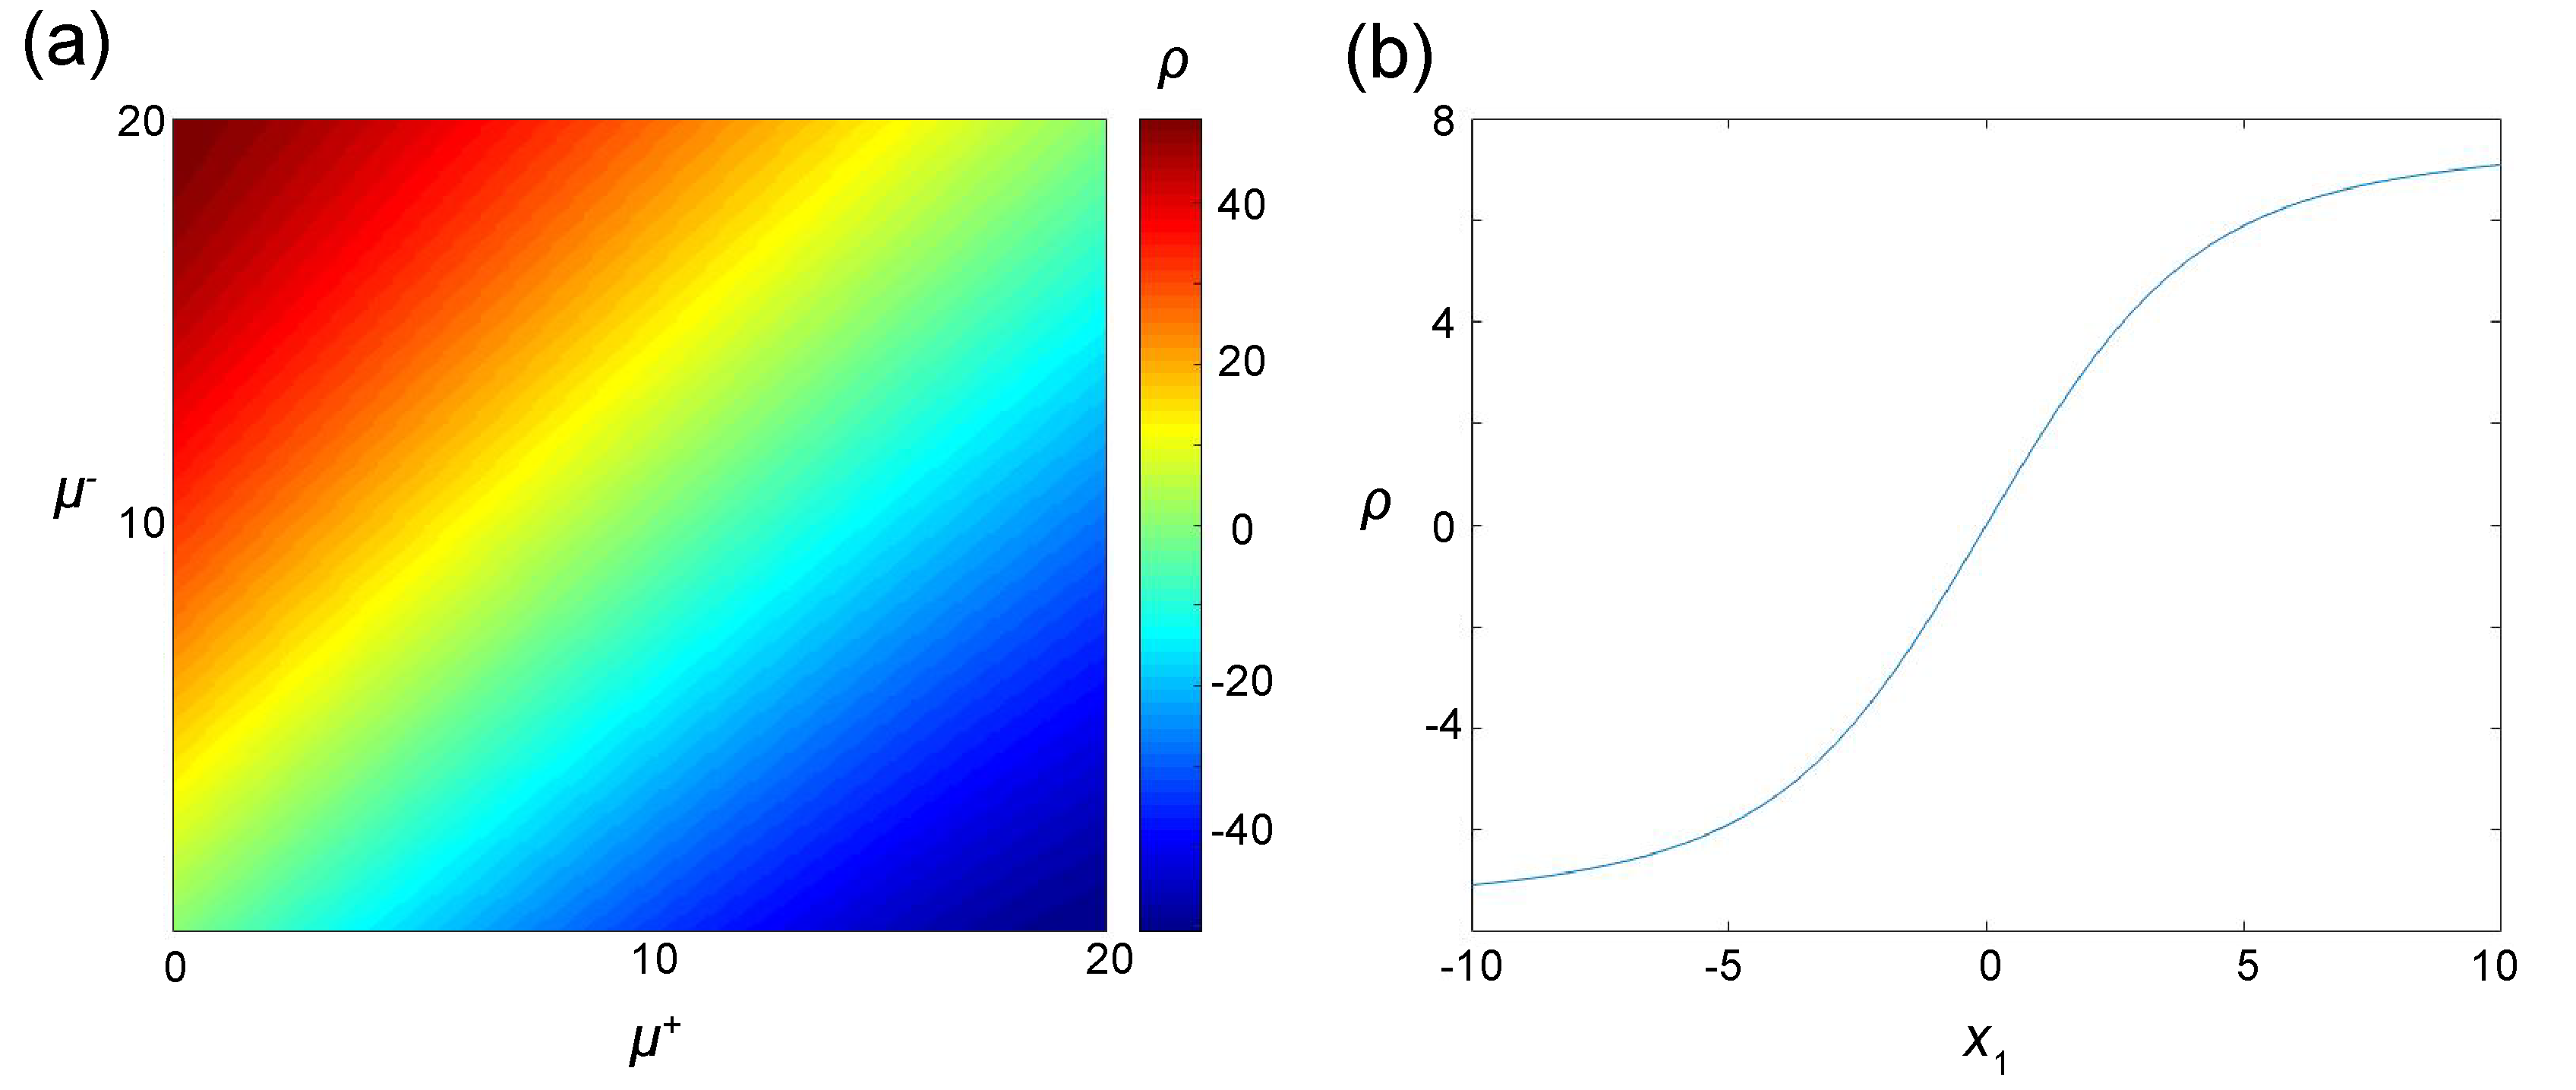
\includegraphics[scale=0.25]{chart/ratefunction.pdf}
	\caption{ST 经验环流和经验净环流的速率函数图像 (a) $\rho=I_Q(\cdots,\mu^+,\mu^-)-I_Q(\cdots,\mu^-,\mu^+)+(\log\frac{\gamma^+}{\gamma^-})(\mu^+-\mu^-)$. (b) $\rho=I_{\tilde{Q}}(\tilde{\mu}^{c_1},\tilde{\mu}^{c_2},\tilde{\mu}^{c_3})- I_{\tilde{Q}}(-\tilde{\mu}^{c_1},\tilde{\mu}^{c_2},\tilde{\mu}^{c_3})
		+(\log\frac{\gamma^{c_1}}{\gamma^{c_1-}})\tilde{\mu}^{c_1}$}\label{figure:ratefunction}
\end{figure}
ST 经验环流无法满足各种涨落定理,ST 经验净环流却是可以在很多情况下成立(参考 \cite{andrieux2007fluctuation,bertini2015flows})。对于单环系统,只需考虑环 $C^+$ 的净环流。从 \eqref{conversion} 式中易知环 $C^+$ 的 ST 经验净环流  $\tilde{Q}^+_n$ 等于 该环的 LE 经验净环流 $\tilde{J}^+_n$。记弦 $l^+$ 和 $l^-$ 分别对应于 $C^+$ 和 $C^-$,由于 $l^+=l^--$,则:
\begin{equation*}\label{circulation}
    \begin{split}
            \tilde{Q}^{+}_n =&\;\sum_{c\in \mathcal{C}}J^c_n1_{\{l^+\in c \}}-\sum_{c\in \mathcal{C}}J^c_n1_{\{l^-\in c \}}\\
            =&\;\sum_{c\in \mathcal{C}}J^c_n1_{\{l^+\in c \}}-\sum_{c\in \mathcal{C}}J^{c-}_n1_{\{l^+\in c \}} = \tilde{J}^+_n.
    \end{split}
\end{equation*}
因此 ST 净环流的涨落定理自然等同于 LE 环流的涨落定理。然而,\eqref{conversion} 式只在周期边界条件下成立,也就意味着,只能得到 ST 经验净环流满足 Gallavotti-Cohen 类型的涨落定理。并且,容易验证 $\tilde{Q}^+_n$ 对其他三种类型的涨落定理不成立。

\BiSection{一般马氏链 LE 环流的涨落定理}{}
目前,已经验证了单环马氏链环流相关的涨落定理,自然会问到环流涨落定理是否会适用于一般的马氏链。下面从回顾文献 \cite{jia2016cycle} 的相关结论开始。记 $c_1=(i_1,i_2,\cdots,i_s)$ 和 $c_2=(j_1,j_2,\cdots,j_r)$ 是两个环。如果 $s=r$ 且 $\{i_1,i_2,\cdots,i_s\}=\{j_1,j_2,\cdots,j_r\}$,则称环 $c_1$ 和环 $c_2$ 相似。
换句话说,如果两个环包含的状态完全一致,则称两个环相似。例如,下面六个环 $(1,2,3,4)$,$(1,2,4,3)$,$(1,3,2,4)$,$(1,3,4,2)$,$(1,4,2,3)$ 和 $(1,4,3,2)$,互为相似关系。根据这个定义,环 $c$ 和它的反环 $c^-$ 一定是相似的。

首先考虑 LE 经验环流 $(J^c_n)_{c\in\mathcal{C}}$。记 $c_1,c_2,\cdots,c_r$ 是一族环,比如,它们可以是环空间中环的全体。若环 $c_s$ 和环 $c_t$ ($1\le s,t\le r$) 相似,那么有下面的暂态涨落定理成立:
\begin{equation}\label{transient}
    \frac{\Pnum(N^{c_s}_n=k^{c_s},N^{c_t}_n=k^{c_t},N^{c_m}_n=k^{c_m},\;\forall m\neq s,t)}
    {\Pnum(N^{c_s}_n=k^{c_t},N^{c_t}_n=k^{c_s},N^{c_m}_n=k^{c_m},\;\forall m\neq s,t)}
    = \left(\frac{\gamma^{c_s}}{\gamma^{c_t}}\right)^{k^{c_s}-k^{c_t}}.
\end{equation}
这表明如果环 $c_s$ 和环 $c_t$ 相似,那么 LE 经验环流的联合分布满足非平凡的对称关系。若环 $c_s$ 和环 $c_t$ 不仅相似,而且互为正反环,则上述方程可以化为:
\begin{equation*}
    \frac{\Pnum(N^+_n=k^+,N^-_n=k^-,N^c_n=k^c,\;\forall c\neq C^+,C^-)}
    {\Pnum(N^+_n=k^-,N^-_n=k^+,N^c_n=k^c,\;\forall c\neq C^+,C^-)}
    = \left(\frac{\gamma^+}{\gamma^-}\right)^{k^+-k^-},
\end{equation*}
这与单环系统的暂态涨落定理有着相同的表达形式。针对从 $i$ 出发的马氏链,并且环 $c_1,c_2,\cdots,c_r$ 通过相同状态 $i\in S$ 的情况,并且文献 \cite{jia2016cycle} 已经给出了 \eqref{transient} 式的有关证明。实际上,使这个结论成立的假设,可以简化为对任意一族环,并且任意初始分布。此外,对任意一族环  $c_1,c_2,\cdots,c_r$ ,任意 $1\le s\le r$,下式成立:
\begin{align*}
&\; \Pnum\left(\tilde{J}^{c_s}_n=x^{c_s}/n,\tilde{J}^{c_m}_n=x^{c_m}/n,\;\forall m\neq s\right) \\
=&\; \Pnum\left(N^{c_s}_n-N^{c_s-}_n=x^{c_s},N^{c_m}_n-N^{c_m-}_n=x^{c_m},\;\forall m\neq s\right) \\
=&\; \sum_{k^{c_m}-k^{c_m-}=x^{c_m},\forall  m }\Pnum\left(N^{c_s}_n=k^{c_s},N^{c_s-}_n=k^{c_s-},  N^{c_m}_n=k^{c_m},N^{c_m-}_n=k^{c_m-},\;\forall m\neq s\right) \\
=&\; \sum_{k^{c_m}-k^{c_m-}=x^{c_m},\forall  m }\Pnum\left(N^{c_s}_n=k^{c_s-},N^{c_s-}_n=k^{c_s}, N^{c_m}_n=k^{c_m},N^{c_m-}_n=k^{c_m-},\;\forall m\neq s\right)\left(\frac{\gamma^{c_s}}{\gamma^{c_s-}}\right)^{k^{c_s}-k^{c_s-}}  \\
=&\; \sum_{k^{c_m}-k^{c_m-}=x^{c_m},\forall  m }\Pnum\left(N^{c_s}_n=k^{c_s-},N^{c_s-}_n=k^{c_s}, N^{c_m}_n=k^{c_m},N^{c_m-}_n=k^{c_m-},\;\forall m\neq s\right)\left(\frac{\gamma^{c_s}}{\gamma^{c_s-}}\right)^{x^{c_s}} \\
=&\; \Pnum\left(N^{c_s}_n-N^{c_s-}_n=-x^{c_s},N^{c_m}_n-N^{c_m-}_n=x^{c_m},\;\forall m\neq s\right)\left(\frac{\gamma^{c_s}}{\gamma^{c_s-}}\right)^{x^{c_s}} \\
=&\; \Pnum\left(\tilde{J}^{c_s}_n=-x^{c_s}/n,\tilde{J}^{c_m}_n=x^{c_m}/n,\;\forall m\neq s\right)\left(\frac{\gamma^{c_s}}{\gamma^{c_s-}}\right)^{x^{c_s}}.
\end{align*}


Thus we finally obtained the following transient fluctuation theorems of empirical LE currents:
\begin{equation}\label{strong}
\Pnum(\tilde{J}^{c_s}_n=x_s,\tilde{J}^{c_m}_n=x_m,\;\forall m\neq s) \\
= \Pnum(\tilde{J}^{c_s}_n=-x_s,\tilde{J}^{c_m}_n=x_m,\;\forall m\neq s)e^{nx_s\log\frac{\gamma^{c_s}}{\gamma^{c_s-}}}.
\end{equation}
This shows that for any cycle $c_s$, the joint distribution of empirical net LE currents satisfies a symmetric relation when $x_s$ is changed to $-x_s$. Note that $\tilde{J}^c_n=0$ for any one-state or two-state cycle $c$ and $\tilde{J}^c_n=-\tilde{J}^{c-}_n$ for any three or more state cycle $c$. Let $c_1,c_1-,c_2,c_2-,\cdots,c_{r*},c_{r*}-$ be all three or more state cycles. If we change $x_s$ to $-x_s$ one by one for $1\leq s\leq r*$ in the above equation, then we obtain
\begin{equation}\label{weak}
\begin{split}
&\;\Pnum\left(\tilde{J}^{c_1}_n=x_1,\tilde{J}^{c_2}_n=x_2,\cdots,\tilde{J}^{c_{r*}}_n=x_{r*}\right)\\
=&\; \Pnum\left(\tilde{J}^{c_1}_n=-x_1,\tilde{J}^{c_2}_n=-x_2,\cdots,\tilde{J}^{c_{r*}}_n=-x_{r*}\right)
e^{n\sum_{i=1}^{r*}x_i\log\frac{\gamma^{c_i}}{\gamma^{c_i-}}}.
\end{split}
\end{equation}
Note that \eqref{weak} is much weaker than \eqref{strong}. As a result, in what follows, we term \eqref{strong} the strong form of the transient fluctuation theorem and term \eqref{weak} the weak form of the transient fluctuation theorem.

Other types of fluctuation theorems for empirical LE and net LE currents can be easily derived from the transient fluctuation theorems and are summarized as follows (here we only show the strong form). For an arbitrary family of cycles $c_1,c_2,\cdots,c_r$, let $g_n(\lambda) = \mathbb{E}[e^{n\sum_{i=1}^r\lambda_iJ^{c_i}_n}]$, $\tilde{g}_n(\lambda) = \mathbb{E}[e^{n\sum_{i=1}^{r}\lambda_i\tilde{J}^{c_i}_n}]$ be the moment generating function of $(J^{c_i}_n)_{1\le i\le r}$, $(\tilde{J}^{c_i}_n)_{1\le i\le r}$ respectively and let $I_{J}(x)$, $I_{\tilde{J}}(x)$ be the rate function of $(J^{c_i}_n)_{1\le i\le r}$, $(\tilde{J}^{c_i}_n)_{1\le i\le r}$ respectively.

Kurchan-Lebowitz-Spohn-type fluctuation theorem: For any cycles $c_s$ and $c_t$ ($1\le s,t\le r$) are similar
\begin{equation*}
	g_n(\cdots,\lambda_s,\cdots,\lambda_t,\cdots) = g_n\left(\cdots,\lambda_t-\log\frac{\gamma^{c_s}}{\gamma^{c_t}},\cdots,\lambda_s+\log\frac{\gamma^{c_s}}{\gamma^{c_t}},\cdots\right).
\end{equation*}
\begin{equation*}
	\tilde{g}_n(\cdots,\lambda_s,\cdots)=\tilde{g}_n\left(\cdots,-\left(\lambda_s+\log\frac{\gamma^{c_s}}{\gamma^{c_s-}}\right),\cdots\right).
\end{equation*}

Integral fluctuation theorem: 
\begin{equation*}
	\mathbb{E}\left[e^{-n\sum_{i=1}^r(\log \gamma^{c_i}/\gamma^{c_i-})\tilde{J}^{c_i}_n}\right]=1.
\end{equation*}

Gallavotti-Cohen-type fluctuation theorem:
\begin{equation*}
	I_J(\cdots,x_s,\cdots,x_t,\cdots)=I_J(\cdots,x_t,\cdots,x_s,\cdots)-\left(\log\frac{\gamma^{c_s}}{\gamma^{c_t}}\right)(x_s-x_t).
\end{equation*}
\begin{equation*}
	I_{\tilde{J}}(\cdots,x_s,\cdots) = I_{\tilde{J}}(\cdots,-x_s,\cdots)-\left(\log\frac{\gamma^{c_s}}{\gamma^{c_s-}}\right)x_s.
\end{equation*}

\subsection{Fluctuation theorems of ST currents for general Markov chains}
We have seen that for monocyclic Markov chains, the empirical ST currents do not satisfy various types of fluctuation theorems, while the empirical net ST currents satisfy the Gallavotti-Cohen-type fluctuation theorems. Next we focus on general Markov chains. It fact, Andrieux and Gaspard \cite{andrieux2007fluctuation} have proved the weak form of Gallavotti-Cohen-type fluctuation theorem for empirical net ST currents: for all three or more state cycles $c_1,c_1-,c_2,c_2-,\cdots,c_r,c_r-$ in the fundamental set $\mathcal{L}$, we have
\begin{equation*}
I_{\tilde{Q}}(x_1,x_2,\cdots,x_r)
= I_{\tilde{Q}}(-x_1,-x_2,\cdots,-x_r)
-\sum_{i=1}^rx_i\log\frac{\gamma^{c_i}}{\gamma^{c_i-}}.
\end{equation*}
This shows that the joint distribution of empirical net ST currents satisfies a symmetric relation when all variables $x_i$ are changed to $-x_i$. 

Interestingly, in contrast to empirical net LE currents, we find that empirical net ST currents do not satisfy the strong form of Gallavotti-Cohen-type fluctuation theorems. To give a counterexample, we consider a four-state Markov chain with a fully connected transition diagram illustrated in Fig. \ref{figure:transitiongraph}(b). Let the spanning tree be $T=1\to2\to3\to4$. Since $\tilde{Q}^{c_l}_n=0$ for all one-state or two-state cycles $c_l$, we only need to consider the rest of the cycles
\begin{equation*}
	c_1 = (1,2,3),\;c_2 = (2,3,4),\;c_3 = (1,2,3,4),\;c_4 = (1,3,2),\;
	c_5 = (2,4,3),\;c_6 = (1,4,3,2).
\end{equation*}
Note that $\tilde{Q}^{c_l}_n=-\tilde{Q}^{c_l-}_n$ for all three or more state cycles and $c_1=c_4-$, $c_2=c_5-$, $c_3=c_6-$. Recall that the rate function of empirical ST currents \eqref{I_Q2}, we have the rate function for $(\tilde{Q}^{c_1}_n,\tilde{Q}^{c_2}_n,\tilde{Q}^{c_3}_n)$ is given by
\begin{equation*}
	I_{\tilde{Q}}(x)=\inf_{\{\mu\in\mathcal{M}:\mu^{c_i}-\mu^{c_i-}= x_i,\forall 1\le i\le 3\}}I_Q(\mu).
\end{equation*}
For cycle $c_1$, if we exchange $\tilde{\mu}^{c_1}$ to $-\tilde{\mu}^{c_1}$, then (see fig. \ref{figure:ratefunction} (b))
\begin{equation*}
I_{\tilde{Q}}(\tilde{\mu}^{c_1},\tilde{\mu}^{c_2},\tilde{\mu}^{c_3})\neq I_{\tilde{Q}}(-\tilde{\mu}^{c_1},\tilde{\mu}^{c_2},\tilde{\mu}^{c_3})
-\left(\log\frac{\gamma^{c_1}}{\gamma^{c_1-}}\right)\tilde{\mu}^{c_1},
\end{equation*}
which shows that the strong form of the Gallavotti-Cohen-type fluctuation theorem fails for empirical net ST currents.